\chapter{Preliminary Analysis}

\section{Shape of the dataset}
The dataset contains:
\begin{itemize}
	\item 891 rows, 
	\item 12 columns.
\end{itemize}


\section{First rows of the dataset} \label{section:first_rows}
An excerpt from the dataset is presented in the table
\ref{table:excerpt_from_dataset}.

\begin{table}[!ht]
	\centering
	\caption{Excerpt from the dataset}
	\resizebox{\textwidth}{!}{
	\begin{tabular}{|r|r|r|r|r|r|r|r|r|r|r|r|r|}
		\hline
		           & \textbf{PassengerId} & \textbf{Survived} & \textbf{Pclass} & \textbf{Name}                                     & \textbf{Sex} & \textbf{Age} & \textbf{SibSp} & \textbf{Parch} & \textbf{Ticket}  & \textbf{Fare} & \textbf{Cabin} & \textbf{Embarked} \\ \hline
		\textbf{0} & 1                    & 0                 & 3               & Braund, Mr. Owen Harris                           & male         & 22.0         & 1              & 0              & A/5 21171        & 7.2500        & NaN            & S                 \\ \hline
		\textbf{1} & 2                    & 1                 & 1               & Cumings, Mrs. John Bradley (Florence Briggs Th... & female       & 38.0         & 1              & 0              & PC 17599         & 71.2833       & C85            & C                 \\ \hline
		\textbf{2} & 3                    & 1                 & 3               & Heikkinen, Miss. Laina                            & female       & 26.0         & 0              & 0              & STON/O2. 3101282 & 7.9250        & NaN            & S                 \\ \hline
		\textbf{3} & 4                    & 1                 & 1               & Futrelle, Mrs. Jacques Heath (Lily May Peel)      & female       & 35.0         & 1              & 0              & 113803           & 53.1000       & C123           & S                 \\ \hline
		\textbf{4} & 5                    & 0                 & 3               & Allen, Mr. William Henry                          & male         & 35.0         & 0              & 0              & 373450           & 8.0500        & NaN            & S                 \\ \hline
	\end{tabular}}
	\label{table:excerpt_from_dataset}
\end{table}

The \textbf{"PassengerId"} feature is the ID of the passanger. It won't 
help in the analysis and will be dropped. Also, there are several missing 
values, and some values are categorical, for example, \textbf{"Pclass"}
and \textbf{"Sex"}.


\section{Data types and missing values}
Table \ref{table:dtypes} contains types of the data in each column and
numbers of non-null values. Table \ref{table:missing_values} contains 
numbers of missing values in each column.

\begin{table}[!ht]
	\centering
	\caption{Data types and non-null counts}
	\begin{tabular}{|l|l|l|l|}
		\hline
		\textbf{\#} & \textbf{Column} & \textbf{Non-Null Count} & \textbf{Dtype} \\ \hline
		\textbf{0}  & PassengerId     & 891 non-null            & int64          \\ \hline
		\textbf{1}  & Survived        & 891 non-null            & int64          \\ \hline
		\textbf{2}  & Pclass          & 891 non-null            & int64          \\ \hline
		\textbf{3}  & Name            & 891 non-null            & object         \\ \hline
		\textbf{4}  & Sex             & 891 non-null            & object         \\ \hline
		\textbf{5}  & Age             & 714 non-null            & float64        \\ \hline
		\textbf{6}  & SibSp           & 891 non-null            & int64          \\ \hline
		\textbf{7}  & Parch           & 891 non-null            & int64          \\ \hline
		\textbf{8}  & Ticket          & 891 non-null            & object         \\ \hline
		\textbf{9}  & Fare            & 891 non-null            & float64        \\ \hline
		\textbf{10} & Cabin           & 204 non-null            & object         \\ \hline
		\textbf{11} & Embarked        & 889 non-null            & object         \\ \hline
	\end{tabular}
	\label{table:dtypes}
\end{table}

\begin{table}[!ht]
	\centering
	\caption{Number of missing values in each column}
	\begin{tabular}{|l|l|l|}
		\hline
		\textbf{\#} & \textbf{Column}   & \textbf{Number of missing values} \\ \hline
		\textbf{0}  & PassengerId       & 0                                 \\ \hline
		\textbf{1}  & Survived          & 0                                 \\ \hline
		\textbf{2}  & Pclass            & 0                                 \\ \hline
		\textbf{3}  & Name              & 0                                 \\ \hline
		\textbf{4}  & Sex               & 0                                 \\ \hline
		\textbf{5}  & \textbf{Age}      & \textbf{177}                      \\ \hline
		\textbf{6}  & SibSp             & 0                                 \\ \hline
		\textbf{7}  & Parch             & 0                                 \\ \hline
		\textbf{8}  & Ticket            & 0                                 \\ \hline
		\textbf{9}  & Fare              & 0                                 \\ \hline
		\textbf{10} & \textbf{Cabin}    & \textbf{687}                      \\ \hline
		\textbf{11} & \textbf{Embarked} & \textbf{2}                        \\ \hline
	\end{tabular}
	\label{table:missing_values}
\end{table}


\pagebreak
\section{Number of unique values}
Table \ref{table:unique_values} contains numbers of unique values in 
each column.

\begin{table}[!ht]
	\centering
	\caption{Number of unique values in each column}
	\resizebox{\textwidth}{!}{
	\begin{tabular}{|
	>{\columncolor[HTML]{EFEFEF}}l |l|
	>{\columncolor[HTML]{EFEFEF}}l |l|}
		\hline
		\textbf{Column} & \textbf{Number of unique values} & \textbf{Column} & \textbf{Number of unique values} \\ \hline
		Name            & 891                              & Survived        & 2                                \\ \hline
		Sex             & 2                                & Pclass          & 3                                \\ \hline
		Ticket          & 681                              & Age             & 88                               \\ \hline
		Cabin           & 147                              & SibSp           & 7                                \\ \hline
		Embarked        & 3                                & Parch           & 7                                \\ \hline
		PassengerId     & 891                              & Fare            & 248                              \\ \hline
	\end{tabular}}
	\label{table:unique_values}
\end{table}

There are high-cardinality features with \textit{object} dtype:
\begin{itemize}
	\item Name
	\item Ticket
	\item Cabin
	\item PassengerId
\end{itemize}
This features, possibly, will need special preprocessing. Earlier, I
noticed that the \textbf{"PassengerId"} feature is the ID of the
passanger. It won't help in the analysis and will be dropped. 

Features \textbf{"Age"} and \textbf{"Fare"} are continuous.


\section{Summary statistics}
In this section, summary statistics for numerical and non-numerical 
attributes are presented in tables \ref{table:numerical_variable_description}
and \ref{table:categorical_variable_description} respectively.

\begin{table}[!ht]
	\centering
	\caption{Summary statistics for numerical attributes}
	\resizebox{\textwidth}{!}{
	\begin{tabular}{|r|r|r|r|r|r|r|r|}
		\hline
		               & \textbf{PassengerId} & \textbf{Survived} & \textbf{Pclass} & \textbf{Age} & \textbf{SibSp} & \textbf{Parch} & \textbf{Fare} \\ \hline
		\textbf{count} & 891.000000           & 891.000000        & 891.000000      & 714.000000   & 891.000000     & 891.000000     & 891.000000    \\ \hline
		\textbf{mean}  & 446.000000           & 0.383838          & 2.308642        & 29.699118    & 0.523008       & 0.381594       & 32.204208     \\ \hline
		\textbf{std}   & 257.353842           & 0.486592          & 0.836071        & 14.526497    & 1.102743       & 0.806057       & 49.693429     \\ \hline
		\textbf{min}   & 1.000000             & 0.000000          & 1.000000        & 0.420000     & 0.000000       & 0.000000       & 0.000000      \\ \hline
		\textbf{25\%}  & 223.500000           & 0.000000          & 2.000000        & 20.125000    & 0.000000       & 0.000000       & 7.910400      \\ \hline
		\textbf{50\%}  & 446.000000           & 0.000000          & 3.000000        & 28.000000    & 0.000000       & 0.000000       & 14.454200     \\ \hline
		\textbf{75\%}  & 668.500000           & 1.000000          & 3.000000        & 38.000000    & 1.000000       & 0.000000       & 31.000000     \\ \hline
		\textbf{max}   & 891.000000           & 1.000000          & 3.000000        & 80.000000    & 8.000000       & 6.000000       & 512.329200    \\ \hline
	\end{tabular}}
	\label{table:numerical_variable_description}
\end{table}

\begin{table}[!ht]
	\centering
	\caption{Summary statistics for non-numerical attributes}
	\begin{tabular}{|r|r|r|r|r|r|}
		\hline
		                & \textbf{Name}           & \textbf{Sex} & \textbf{Ticket} & \textbf{Cabin} & \textbf{Embarked} \\ \hline
		\textbf{count}  & 891                     & 891          & 891             & 204            & 889               \\ \hline
		\textbf{unique} & 891                     & 2            & 681             & 147            & 3                 \\ \hline
		\textbf{top}    & Braund, Mr. Owen Harris & male         & 347082          & B96 B98        & S                 \\ \hline
		\textbf{freq}   & 1                       & 577          & 7               & 4              & 644               \\ \hline
	\end{tabular}
	\label{table:categorical_variable_description}
\end{table}


\section{Proportion of target values}

Let's check if one class of target values is more frequent than another.

Figure \ref{number_of_survivors} illustrates these numbers. There are 342 
(38.38\%) survived passengers and 549 (61.62\%) drowned passengers in the 
dataset, so the dataset is a bit skewed. Therefore, the accuracy may not be 
sufficient to assess the performance of classifiers.

\begin{figure}[!ht]
	\centering
	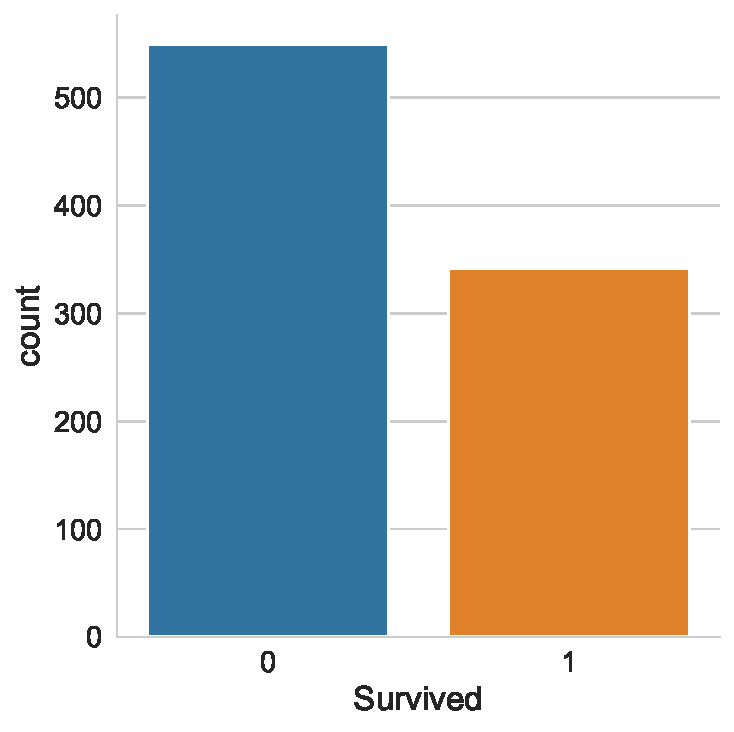
\includegraphics[width=0.5\textwidth]{number_of_survivors}
	\caption{Number of survived and drowned passangers in whole dataset}
	\label{number_of_survivors}
\end{figure}